\documentclass[t]{beamer}  % [t], [c], или [b] --- вертикальное выравнивание на слайдах (верх, центр, низ)
%\documentclass[handout]{beamer} % Раздаточный материал (на слайдах всё сразу)
%\documentclass[aspectratio=169]{beamer} % Соотношение сторон

\usetheme{PaloAlto} % Тема оформления
%\usetheme{Bergen}
%\usetheme{Szeged}

\usecolortheme{wolverine} % Цветовая схема
%\useinnertheme{circles}
%\useinnertheme{rectangles}

%\usetheme{HSE}

%%% Работа с русским языком
\usepackage{cmap}					% поиск в PDF
\usepackage{mathtext} 				% русские буквы в формулах
\usepackage[T2A]{fontenc}			% кодировка
\usepackage[utf8]{inputenc}			% кодировка исходного текста
\usepackage[english,russian]{babel}	% локализация и переносы

%% Beamer по-русски
\newtheorem{rtheorem}{Теорема}
\newtheorem{rproof}{Доказательство}
\newtheorem{rexample}{Пример}

%%% Дополнительная работа с математикой
\usepackage{amsmath,amsfonts,amssymb,amsthm,mathtools} % AMS
\usepackage{icomma} % "Умная" запятая: $0,2$ --- число, $0, 2$ --- перечисление

%% Номера формул
%\mathtoolsset{showonlyrefs=true} % Показывать номера только у тех формул, на которые есть \eqref{} в тексте.
%\usepackage{leqno} % Нумерация формул слева

%% Свои команды
\DeclareMathOperator{\sgn}{\mathop{sgn}}

%% Перенос знаков в формулах (по Львовскому)
\newcommand*{\hm}[1]{#1\nobreak\discretionary{}
{\hbox{$\mathsurround=0pt #1$}}{}}

%%% Работа с картинками
\usepackage{graphicx}  % Для вставки рисунков
%\setlength\fboxsep{3pt} % Отступ рамки \fbox{} от рисунка
%\setlength\fboxrule{1pt} % Толщина линий рамки \fbox{}
%\usepackage{wrapfig} % Обтекание рисунков текстом

%%% Работа с таблицами
\usepackage{array,tabularx,tabulary,booktabs} % Дополнительная работа с таблицами
\usepackage{longtable}  % Длинные таблицы
\usepackage{multirow} % Слияние строк в таблице

%%% Программирование
\usepackage{etoolbox} % логические операторы

%%% Другие пакеты
\usepackage{lastpage} % Узнать, сколько всего страниц в документе.
\usepackage{soul} % Модификаторы начертания
\usepackage{csquotes} % Еще инструменты для ссылок
%\usepackage[style=authoryear,maxcitenames=2,backend=biber,sorting=nty]{biblatex}
\usepackage{multicol} % Несколько колонок

%%% Картинки
\usepackage{tikz} % Работа с графикой
\usepackage{pgfplots}
\usepackage{pgfplotstable}

\title{ Презентация: Сдача экзамена по информатике}
%\subtitle{}
\author{Авсюкеви Станислав}
\date{\today}
\institute[ЛЭТИ]{Ленинградский Электротехнический Институт (Им. В. И. Ульянова (Ленина))<<ЛЭТИ>>}

\begin{document}

\maketitle
%\frame[plain]{\titlepage}	% Титульный слайд

\section{Оглавление}
%\subsection{Команда pause}

\begin{frame}
	\frametitle{\insertsection} 
\tableofcontents
	
\end{frame}
 
\section{Всемирная паутина (WWW)}
\subsection{Введение}

\begin{frame}
	\frametitle{\insertsection} 
	\framesubtitle{\insertsubsection}

	\parindent=1cm \alert{ Интернет} — это сеть сетей, обеспечивающая инфраструктуру для взаимодействия и совместного использования информации. \only<2->{ Он обеспечивает ряд сервисов, такие как электронная почта, передача файлов, подключение в режиме удаленного терминала, интерактивные конференции, группы новостей, и WWW. }

\begin{figure}
\begin{center}
\begin{minipage}[h]{0.5\linewidth}
\center{\includegraphics[width=1\linewidth]{1.jpg}}  \\
\end{minipage}
\end{center}
\end{figure}

\end{frame}

\subsection{World Wide Wed}

\begin{frame}
	\frametitle{\insertsection} 
	\framesubtitle{\insertsubsection}
	
 \only<2>{\parindent=1cm \alert{World Wide Web} — это вселенная информации, доступная из Интернета. WWW появился как сетевой информационный проект в CERN, европейской физической лаборатории.}

\begin{figure}
\begin{center}
\begin{minipage}[h]{0.85\linewidth}
\center{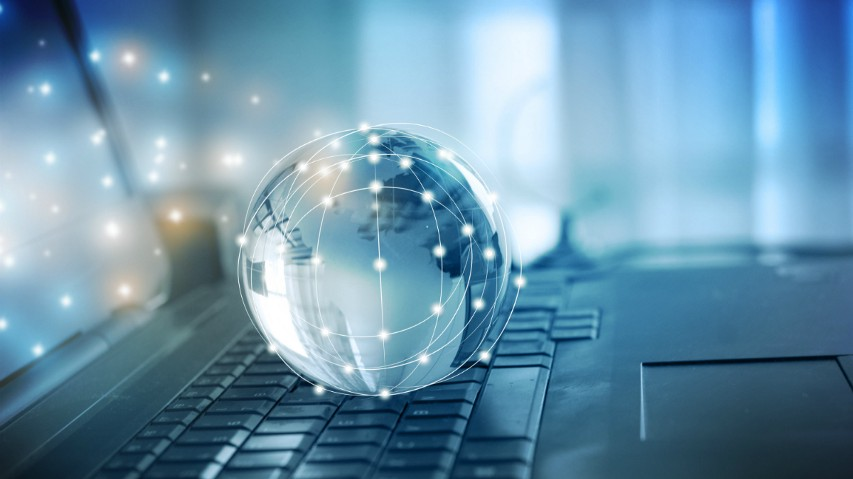
\includegraphics[width=1\linewidth]{2.jpg}}  \\
\end{minipage}
\end{center}
\end{figure}

\end{frame}

\subsection{История}

\begin{frame}
	\frametitle{\insertsection} 
	\framesubtitle{\insertsubsection}

 \only<1>{
\begin{figure}
\begin{center}
\begin{minipage}[h]{0.85\linewidth}
\center{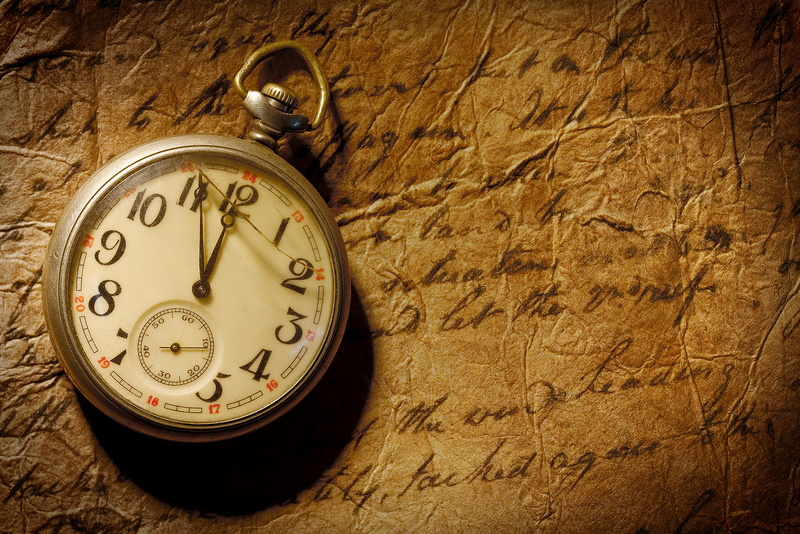
\includegraphics[width=1\linewidth]{3.jpg}}  \\
\end{minipage}
\end{center}
\end{figure}}	
  \only<2->{\begin{itemize} 
\item 1960 г. - Тед Нельсон продвигал идеею связывания документов через гипертекст;
\item 1969 г. - Министерство обороны США;
\item 1972 г. - открыт доступ для университетов(50 шт.);
\item 1973 г. - международные масштабы (объединение сетей Англии и Норвегии);
\item 1990 г. - представлен первый текстовый браузер (browser).
\item 1993 г. - выход первой Unix-версии графического браузера «Mosaic»;
\item 1994 г. - создание браузеров для операционных систем Windows и Macintosh (Netscape Navigator и Microsoft Internet Explorer)
\end{itemize}}

\end{frame}

\subsection{Кратко о работе}

\begin{frame}
	\frametitle{\insertsection} 
	\framesubtitle{\insertsubsection}
	\parindent=1cm \alert{Технология WWW} позволяет создавать гиперссылки, которые реализуют переходы не только внутри исходного документа, но и на любой другой документ, находящийся на другом компьютере, подключенном в данный момент к Интернету.

\begin{figure}
\begin{center}
\begin{minipage}[h]{0.5\linewidth}
\center{
\includegraphics[width=1\linewidth]{4.jpg}}  \\
\end{minipage}
\end{center}
\end{figure}

\end{frame}

\begin{frame}
	\frametitle{\insertsection} 
	\framesubtitle{\insertsubsection}
	\parindent=1cm \alert{Система WWW} построена на специальном протоколе передачи данных, который называется протоколом передачи гипертекста HTTP.

\parindent=1cm Всё содержимое системы WWW состоит из WWW-страниц.
\begin{figure}
\begin{center}
\begin{minipage}[h]{0.7\linewidth}
\center{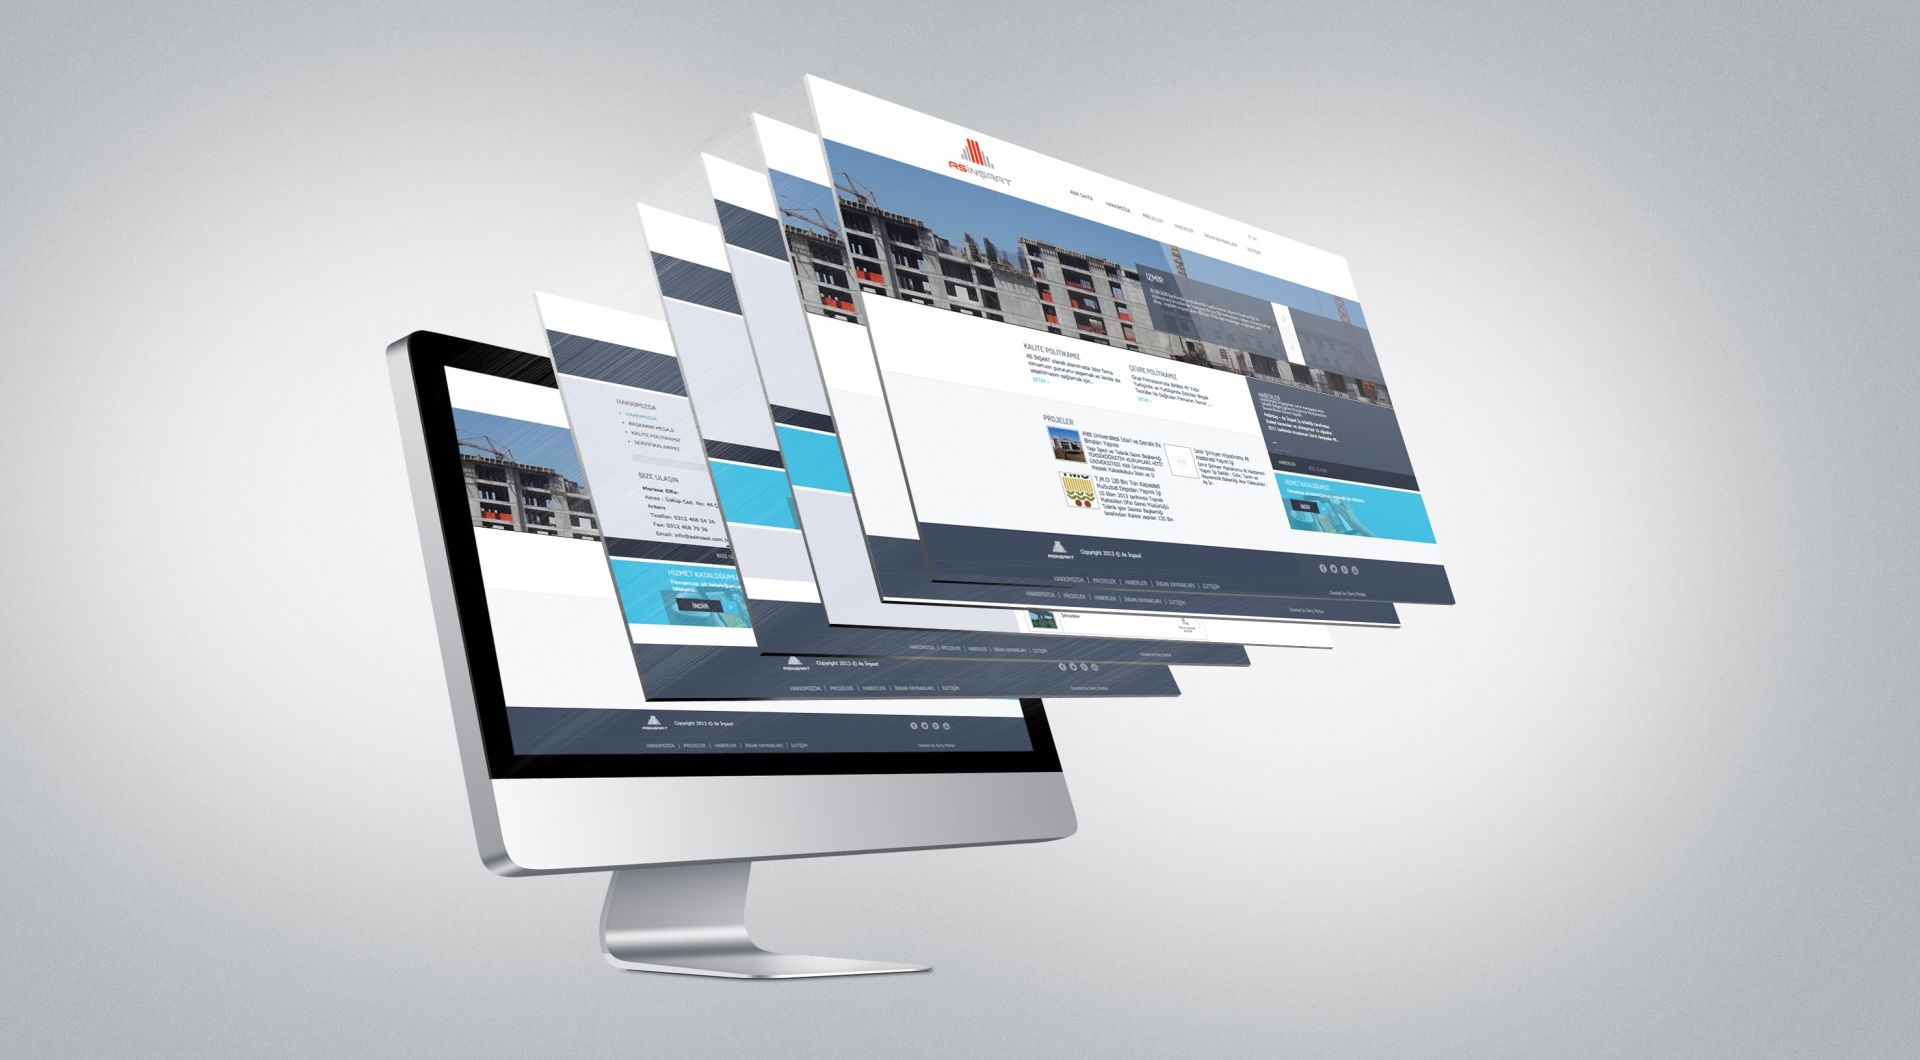
\includegraphics[width=1\linewidth]{5.jpg}}  \\
\end{minipage}
\end{center}
\end{figure}
	
\end{frame}

\section{Интерполяция функции кубическим сплайном}
\subsection{Определение}

\begin{frame}
	\frametitle{\insertsection} 
	\framesubtitle{\insertsubsection}
	\parindent=1cm \alert{Интерполяция} - нахождение промежуточных значений функции по некоторым известным ее значениям. 

 \begin{figure}
\begin{center}
\begin{tikzpicture}
\begin{scope}[xscale=2, yscale=1]

\draw[thin, ->] (-1,0) -- (3.5,0) node[right] {$X$};
\draw[thin, ->] (0,-1) -- (0,3) node[left] {$Y$};

\draw[domain=0:0.25, smooth, purple] plot ({\x},{4.856*(\x)*(\x)*(\x)+0*(\x)*(\x)-1.9035*(\x)+2});
\draw[domain=0.25:1.25, smooth, purple] plot ({\x},{-1.924*(\x)*(\x)*(\x)+5.085*(\x)*(\x)-3.1748*(\x)+2.1059});
\draw[domain=1.25:2.125, smooth, purple] plot ({\x},{1.2968*(\x)*(\x)*(\x)-6.9929*(\x)*(\x)+11.9227*(\x)-4.1847});
\draw[domain=2.125:3.25, smooth, purple] plot ({\x},{-0.3775*(\x)*(\x)*(\x)+3.6803*(\x)*(\x)-10.7579*(\x)+11.8808});

\draw[thin,blue,dashed] (0.25, 1.6) -- (0.25, 0) node [below] {$0.25$};
\draw[thin,blue,dashed] (1.25, 2.325) -- (1.25, 0) node [below] {$1.25$};
\draw[thin,blue,dashed] (2.125, 2.017) -- (2.125, 0) node [below] {$2.125$};
\draw[thin,blue,dashed] (3.25, 2.833) -- (3.25, 0) node [below] {$3.25$};
%\draw[thin,blue,dashed] (3.25, 2.833) -- (3.25, 0) node [below] {$3.25$};


\filldraw ( 0, 2) circle (0.05cm) node [above,left] {$A(0,2)$};
\filldraw (0.25, 1.6) circle (0.05cm) node [below=15pt,right] {$B(0.25, 1.6)$};
\filldraw (1.25, 2.325) circle (0.05cm) node [above=15pt,right] {$C(1.25, 2.325)$};
\filldraw (2.125, 2.017) circle (0.05cm) node [below=25pt,right] {$D(2.125, 2.017)$};
\filldraw (3.25, 2.833) circle (0.05cm) node [right] {$I(3.25, 2.833)$};
	
%\draw[domain=0:0.25, smooth, purple] plot ({\x},{4.8004341681*(\x)*(\x)*(\x)+0*(\x)*(\x)-1.900027198*(\x)+2});
%\draw[domain=0.25:1.25, smooth, purple] plot ({\x},{-1.87538007721*(\x)*(\x)*(\x)+5.0068619551*(\x)*(\x)-3.1517426868*(\x)+2.1043096241});
%\draw[domain=1.25:2.125, smooth, purple] plot ({\x},{1.1050110899*(\x)*(\x)*(\x)-6.169075272*(\x)*(\x)+10.8188441661*(\x)-3.7167682313});
%\draw[domain=2.125:3.25, smooth, purple] plot ({\x},{0.137229517*(\x)*(\x)*(\x)+0*(\x)*(\x)-2.2915718292*(\x)+5.569776432});

\end{scope};
\end{tikzpicture}
\caption{График функции кубического сплайна} \label{graf6}
\end{center}
\end{figure}

\end{frame}

\begin{frame}
	\frametitle{\insertsection}
	\framesubtitle{\insertsubsection}
\begin{figure}
\begin{center}
\begin{minipage}[h]{0.9\linewidth}
\center{
\includegraphics[width=1\linewidth]{6.jpg}}  \\
\end{minipage}
\end{center}
\end{figure}

\end{frame}

\subsection{Получймая погрешность}

\begin{frame}
	\frametitle{\insertsection}
	\framesubtitle{\insertsubsection}
\parindent=1cm Полученная погрешность в результате интерполяции  кубическим сплайном:
  $
\left | S_3^{(r)}(x) - f^{(r)}(x) \right | \leqslant \color<2->[RGB]{255,45,0}1.0555 \times 10^{-6}.
$
\begin{figure}
\begin{center}
\begin{minipage}[h]{0.5\linewidth}
\center{
\includegraphics[width=1\linewidth]{7.png}}  \\
\end{minipage}
\end{center}
\end{figure}

\end{frame}

\begin{frame}
\begin{figure}
\begin{center}
\begin{minipage}[h]{1\linewidth}
\center{
\includegraphics[width=1\linewidth]{8.jpg}}  \\
\end{minipage}
\end{center}
\end{figure}

\end{frame}


\end{document}